\documentclass[11pt]{article}
\usepackage[margin=1in]{geometry}
\usepackage{amsmath,amssymb}
\usepackage{graphicx}
\usepackage[hidelinks]{hyperref}

\title{Literature Status: Greedy-Envelope Counterexamples}
\author{Automatic Math Discovery Run \texttt{fa\_banach\_001}}
\date{June 12, 2026}

\begin{document}
\maketitle

\section*{Original Problems}

The original source is Fernando Albiac, Jos\'e L. Ansorena, Pablo M. Bern\'a,
and Przemys{\l}aw Wojtaszczyk,
\emph{Greedy approximation for biorthogonal systems in quasi-Banach spaces},
arXiv:1903.11651; Dissertationes Mathematicae 560 (2021), 1--88.

In the arXiv PDF, the relevant questions appear as Problems 12.5 and 12.6.
Problem 12.5 contains the general Banach-envelope question and a more
special bidemocratic refinement:

\begin{center}

\includegraphics[width=\textwidth]{figures/open_problem_crop.png}
\end{center}

Problem 12.6 contains the reordering question:

\begin{center}
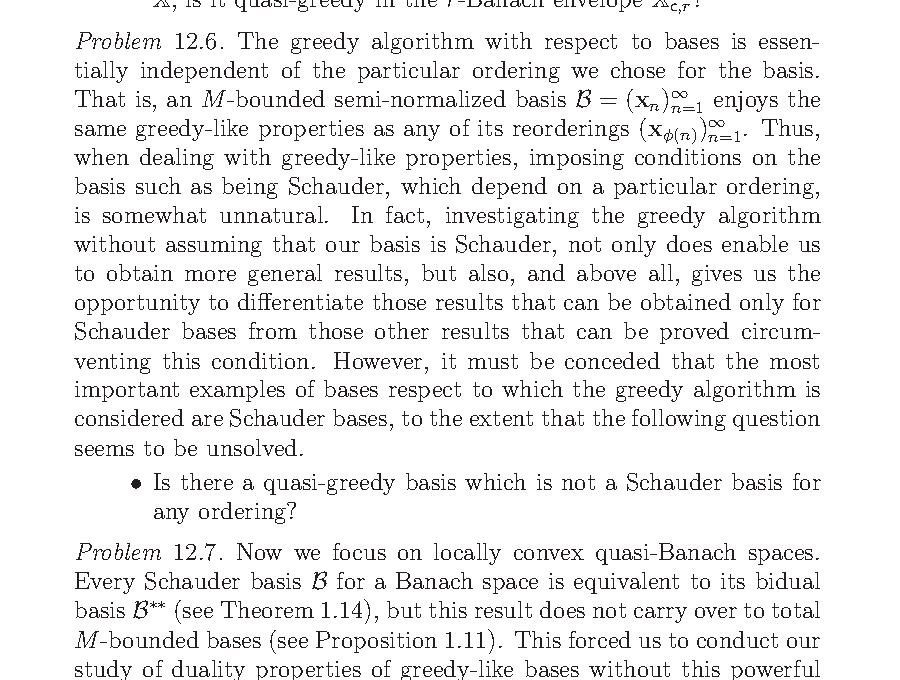
\includegraphics[width=\textwidth]{figures/open_problem_12_6_crop.png}
\end{center}

The first question asks, in its general part, whether a quasi-greedy basis in a
quasi-Banach space remains quasi-greedy when passed to the Banach envelope.
The second asks whether there can be a quasi-greedy basis which is not a
Schauder basis for any ordering.

\section*{Supporting Answer Source}

The supporting paper is Fernando Albiac, Jos\'e L. Ansorena, Miguel
Berasategui, and Pablo M. Bern\'a,
\emph{When Greedy Approximation Breaks: Counterexamples in Quasi-Banach
Spaces}, arXiv:2510.13693.

It cites the same questions using the published numbering as AABW Problems
13.5 and 13.6, and the AAT 2025 survey numbering as Problems 16 and 14:

\begin{center}

\includegraphics[width=\textwidth]{figures/supporting_answer_crop.png}
\end{center}

\section*{Answer}

The questions checked in this packet are already answered in the negative by
arXiv:2510.13693.

\begin{itemize}
\item Question A / AABW Problem 13.5 / AAT Problem 16 has a negative answer:
there exists a quasi-Banach space \(X\) with an almost greedy Schauder basis
whose image in the Banach envelope of \(X\) is not quasi-greedy.

\item Question B / AABW Problem 13.6 / AAT Problem 14 has a positive
existence answer: there exists a quasi-Banach space with an almost greedy
basis which fails to be a Schauder basis under every rearrangement. Since an
almost greedy basis is quasi-greedy, this answers the original quasi-greedy
ordering question.
\end{itemize}

\section*{Verification Notes}

The local source file
\[
\texttt{data/parsed/arxiv\_sources/2510.13693/GreedyEnvelopeV02.tex}
\]
contains the following checks:

\begin{itemize}
\item lines 142--151 restate Question A and Question B and state that the
paper gives counterexamples resolving both problems;
\item the theorem collected near line 999 constructs the Banach-envelope
counterexample and is followed by the sentence that it solves Question A in
the negative;
\item Theorem \texttt{thm:AMain}, around lines 1406--1416, constructs an
almost greedy basis failing to be a Schauder basis under any rearrangement,
thereby answering Question B in the negative.
\end{itemize}

\section*{Limitations}

This packet is a literature-status packet, not an original proof or a new
counterexample produced by this run. It also does not claim the bidemocratic
refinement inside the original Problem 12.5, since the supporting paper's
Question A is the general Banach-envelope problem. Finally, the supporting
paper notes that the ordering question remains open when restricted to Banach
spaces.

\section*{Search Bounds}

The local run registry, solution packets, and attempts were searched for
arXiv:2510.13693, the title phrase, the Banach-envelope quasi-greedy question,
and Problems 13.5 and 13.6. No existing packet or registry row was found.
Web search on June 12, 2026 located the arXiv records for arXiv:1903.11651,
arXiv:2405.20939, and arXiv:2510.13693; the latter explicitly states in its
abstract and introduction that it resolves the two earlier problems.

\section*{Human Review Recommendation}

Reviewers should check the numbering mismatch between the arXiv preprint
Problems 12.5--12.6 and the published AABW numbering cited by the answer paper
as Problems 13.5--13.6. They should also verify that the packet is restricted
to the general envelope question and the quasi-Banach ordering question, not
to the bidemocratic subproblem or the Banach-space-only variant.

\end{document}
